\documentclass[a4paper,10pt]{article}
\usepackage{amsmath,amssymb,graphicx,float,subfig}

%defines
\def\bY{{\bf Y}}
\def\bA{{\bf A}}
\def\bB{{\bf B}}
\def\bX{{\bf X}}
\def\bH{{\bf H}}
\def\bE{{\bf E}}
\def\bG{{\bf G}}
\def\bV{{\bf V}}
\def\bQ{{\bf Q}}
\def\btQ{{\bf \tilde Q}}
\def\bC{{\bf C}}
\def\btA{{\bf \tilde A}}
\def\b1{{\bf 1}}
\def\bx{{\bf x}}
\def\bb{{\bf b}}
\def\be{{\bf e}}
\def\by{{\bf y}}
\def\bz{{\bf z}}
\def\btx{{\bf{\tilde x}}}
\def\blambda{{\boldsymbol \lambda}}
\def\bgamma{{\boldsymbol \gamma}}
\def\btheta{{\boldsymbol \theta}}
\def\bbeta{{\boldsymbol \beta}}
\def\bnu{{\boldsymbol \nu}}
\def\bmu{{\boldsymbol \mu}}
\def\sigmaeps{{\sigma_{\epsilon}}}
\def\bxmode{{\hat \bx^{(0)}}}
\def\txmode{{\tilde \bx_{\mathrm{mode}}}}
\def\txsample{{\tilde \bx_{\mathrm{sample}}}}

%opening
\title{Home Assignment - 2}
\author{Santhosh Nadig, Zhanzhang Cai}

\begin{document}

\maketitle

\section{Introduction}
Non-Gaussian data is common and widly exists in nature, such as number of forest fires happens (count data), area of forest pest infestation occur (0/1), precipitation (positive). Sptatially reconstructing these non-Gaussian data is important to understand and modeling their procedure. In this assignment, as a case study, we will use the monthly (2011-06) precipitation observations in the Parana district of Brazil, and based on elevation and distance to coast, to reconstruct spatially consecutive precipitation map for the region.  

\section{The Data-Set and Model}
\label{sec:model}
The data consists of precipitation for the month of June, 2011 for 553 locations in the Parana district of Brazil. In addition, we are given the co-ordinates (latitude, longitude), elevation and distance to the coast are provided. The data is positive (since it is the accumulated precipitation) and the following model is suggested.

\begin{itemize}
 \item The observations $y_i$ are Gamma distributed
 \begin{align*}
  & y_i|z_i \sim \Gamma \left( b , \frac{e^{z_i}}{b}\right) \\
  & p(y_i|z_i) = \frac{y_i^{b-1}}{\Gamma(b)} \left( b e^{-z_i} \right)^b \exp(b y_i e^{-z_i})
 \end{align*}
 The mean $E(y_i|z_i) = e^{z_i}$ and $\log E(y_i|z_i) = z_i$. And, the variance $V(y_i|z_i) = e^{2z_i}/b$.
 
 \item The log-expectation of the observations $\bz$ is modeled as 
 \begin{align*}
  & \bz = \bA \bx + \bB \bbeta = \btA \btx.
 \end{align*}
 where $\bA$ is the observation matrix, $\bB$ is a matrix of covariates and
 \begin{align*}
  &\btx = \begin{bmatrix}
          \bx \\
          \bbeta
         \end{bmatrix} \sim
         N\left( 0, \begin{bmatrix}
                     \bQ & 0 \\
                     0 & \mathbb{I} \cdot 10^{-3}
                    \end{bmatrix}^{-1}
 \right)
 \end{align*}
 \item A suitable model for $\bQ$ is a SAR model: $\bQ = \tau (\kappa^4 \bC + 2\kappa^2 \bG + \bG_2)$ with parameters $\theta_1 = \log (\tau)$,  $\theta_2 = \log (\kappa^2)$  and $\theta_3 = \log(b)$.
\end{itemize}


\section{Theory}
\subsection{Observation Log-Likelihood}
The data model is given by
\begin{equation}
 p(y_i|z_i) = \frac{y_i^{b-1}}{\Gamma(b)} (be^{-z_i})^b \exp (-by_ie^{-z_i}).
 \label{eq:datamodel}
\end{equation}
Thus, the observation log-likelihood $\log p(y_i|z_i)$ can be written as
\begin{equation*}
 f(z_i) \triangleq \log p(y_i|z_i) = (b-1) \log y_i - \log \Gamma(b) + b \log (b) - b z_i - b y_i e^{-z_i},
\end{equation*}
whose derivatives are
\begin{align*}
 f'(z_i) &= -b + b z_i y_i e^{-z_i} \\
 f''(z_i) &= b y_i e^{-z_i} (1 - z_i) .
\end{align*}

\subsection{Log-likelihood $\log p(\btx|\by, \btheta)$}
The log-likelihood function $\log p(\btx|\by, \btheta)$ can be written as
\begin{align}
 \log p(\btx|\by, \btheta) &\propto \log p(\by| \btx, \btheta) + \log p(\btx|\btheta) + \mathrm{const.} \nonumber \\
 &= \sum_i \log p(y_i|z_i, \btheta) + \log p(\btx|\btheta) + \mathrm{const.} \nonumber \\
 &= \sum_i f(z_i) - \frac{1}{2} \btx^T \bQ \btx  + \mathrm{const.}
 \label{eq:logpxyt}
\end{align}
The Taylor expansion around the mode $\hat \bx^{(0)}$ of the first term $\sum_i f(z_i)$ is given by [slide 29 of lecture 7]
\begin{equation}
 \sum_i f(z_i) \approx \mathrm{const.} + \btx^T \btA^T (\nabla f^{(0)} - \bH_f^{(0)} \btA \hat \bx^{(0)}) + \frac{1}{2} \btx^T \btA^T \bH_f^{(0)} \btA \btx
 \label{eq:taylor}
\end{equation}
where $\nabla f^{(0)}$ and $\bH_f^{(0)}$ represent the gradient and Hessian of $f$ at the mode of $\btx$.
Substituting (\ref{eq:taylor}) in (\ref{eq:logpxyt}), one obtains
\begin{equation}
 g(\btx) \triangleq \log p(\btx|\by, \btheta) \approx \btx^T \bb_{x|y} - \frac{1}{2} \btx^T \bQ_{x|y} \btx,
 \label{eq:gx}
\end{equation}
where $\bb_{x|y} = \btA^T (\nabla f^{(0)} - \bH_f^{(0)} \btA \hat \bx^{(0)})$ and $\bQ_{x|y} = \btQ - \btA^T \bH_f^{(0)} \btA$.

Taking the first derivative w.r.t $\btx$ of (\ref{eq:gx}), one obtains
\begin{align}
 g'(\btx) &= \btA^T (\nabla f^{(0)} - \bH_f^{(0)} \btA \hat \bx^{(0)}) - (\btQ - \btA^T \bH_f^{(0)} \btA) \btx \nonumber \\
	  &= \btA^T \nabla f^{(0)} - \btQ \hat \bx^{(0)} \qquad \mathrm{at~} \btx = \hat \bx^{(0)}.
\end{align}
The second derivative w.r.t $\btx$ of (\ref{eq:gx}) can simply be written as
\begin{equation}
 g''(\btx) = -(\btQ - \btA^T \bH_f^{(0)} \btA).
\end{equation}

Furthermore, comparing equation (\ref{eq:gx}) to a canonical multivariate Gaussian log-likelihood function, the Gaussian approximation of $p(\btx|\by, \btheta)$ [slide 32 of lecture 7] can be obtained as,
\begin{align}
 p_G(\btx|\by, \btheta) &\stackrel{\in}{\sim} N(\bmu_{x|y}, \bQ_{x|y}^{-1}) \nonumber \\
 \bmu_{x|y} &= \bQ_{x|y}^{-1} \bb_{x|y}
 \label{eq:pxygauss}
\end{align}

\section{Estimation}
The observations are divided into estimation and validation data-sets wherein approximately 10\% of the observations are set aside for validation.
\subsection{Ordinary Least Squares}
The model for ordinary least squares is given by
\begin{equation*}
 \bz = \bB \bbeta + \be
\end{equation*}
where $\bB$ represents the matrix of covariates, $\bbeta$ the vector of coefficients and $\be \sim N(0,\sigmaeps^2)$.

The first step is to select a suitable set of covariates. Towards this end, a set of models tabulated in table \ref{tab:models} are explored.
\begin{table}[H]
\centering
\begin{tabular}{lp{9cm}}
\hline
{\bf Model} & {\bf Covariates} \\
\hline
 A & Latitude, longitude, distance to coast, elevation\\
 * B & Latitude, distance to coast, elevation\\
 C & Distance to coast, elevation\\
 D & Longitude, distance to coast\\
 E & Longitude, elevation\\
\hline
\end{tabular}
\caption{Models and the respective covariates, with log precipitation as the independent varible.}
\label{tab:models}
\end{table}

The standard error of the residuals and Akaike Information Criterion (AIC) for the models are shown in figure \ref{fig:aicse}. Clearly, model B is the best choice. Thus, the covariates include an intercept ($\beta_0$), latitude, distance to coast and elevation.
\begin{figure}[ht]
\centering
  \subfloat[]{{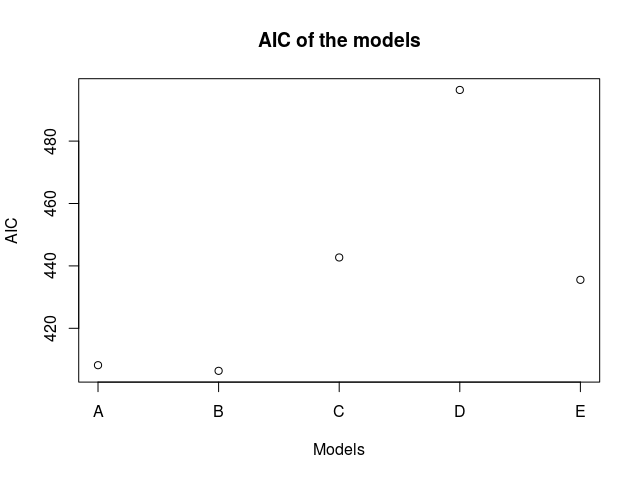
\includegraphics[width=5cm, height=5cm]{AIC_mm.png} }}%
  \qquad
  \subfloat[]{{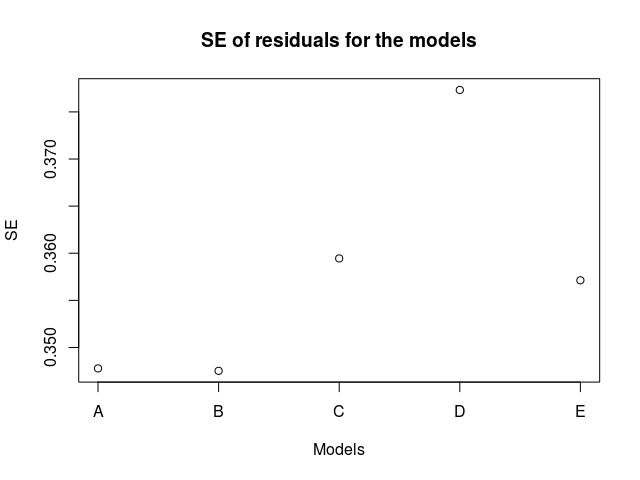
\includegraphics[width=5cm, height=5cm]{SE_Resid_mm.png} }}%
  \caption{(a): AIC (b): SE of residuals.}
\label{fig:aicse}
\end{figure}

The estimated parameters $\hat \bbeta$ and their corresponding standard errors tabulated in table~\ref{tab:olsparest}. The estimated noise variance was $\sigmaeps^2 = 0.1069$.
\begin{table}[H]
\centering
\begin{tabular}{lll}
\hline
{\bf Parameter} & {\bf Estimate} & {\bf SE} \\
\hline
$\hat \beta_0$ & -10.8703 & 1.9788 \\
$\hat \beta_1$ & -0.2430 & 0.0413 \\
$\hat \beta_2$ & -0.2234 & 0.0429 \\
$\hat \beta_3$ & 0.0006 & 0.0001 \\
\hline
\end{tabular}
\caption{OLS parameter estimate and standard errors.}
\label{tab:olsparest}
\end{table}

The OLS estimate of the expected value of precipitation at the validation locations is simply given by $\bE(\hat \by_v) = \hat \bmu_v = \exp \left( \bB_v \hat \bbeta \right)$, where $\bB_v$ is the covariate matrix for the validation locations. Furthermore, the variance of the expected precipitation is given by $\bV(\hat \bmu_v) = \sigmaeps^2 (\bB_v (\bB_v^T\bB_v)^{-1} \bB_v^T)$. The 95\% confidence intervals (Gaussian) are given by $\hat \bmu_v \pm 1.96 \left( \bV(\hat \bmu_v) \right)^{1/2}$.

The OLS estimate for the validation locations, along with the 95\% confidence intervals are plotted in figure~\ref{fig:valid} (a).
\begin{figure}[ht]
\centering
  \subfloat[]{{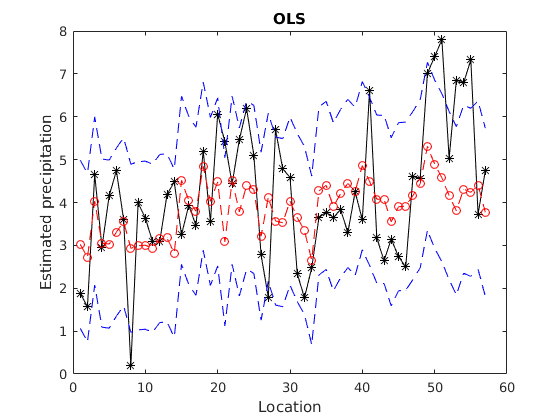
\includegraphics[width=5cm, height=4.5cm]{ols_valid.png} }}%
  \qquad
  \subfloat[]{{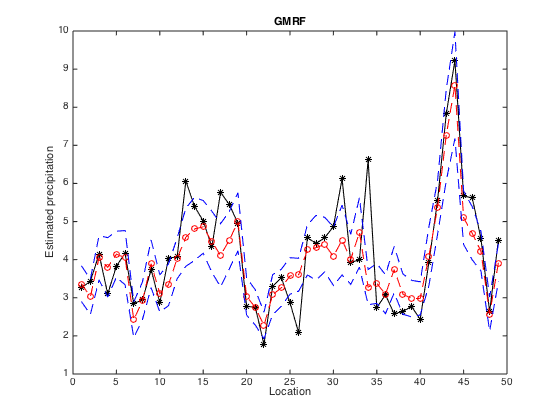
\includegraphics[width=5cm, height=4.5cm]{gmrf_valid.png} }}%
  \caption{(a): OLS estimate of expected precipitation at the validation locations. (b): GMRF estimate of precipitation at the validation locations.\\ Black: Truth, Red: estimate of expected precipitation, Blue: 95\% confidence intervals.}
\label{fig:valid}
\end{figure}

\subsection{Gaussian Markov Random Field (GMRF)}

We begin by estimatating the parameters of the GMRF model described in section \ref{sec:model} for which we require the posterior $p(\btheta|\by)$. The parameter estimates are obtained as,
\begin{equation*}
 \hat \btheta = \arg\max_{\btheta} \, p(\btheta|\by)
\end{equation*}
Since we assume $p(\btheta) \propto 1$ (``flat-prior''), we may express the posterior as
\begin{align*}
 p(\btheta|\by) \propto p(\by|\btheta) &= \frac{p(\by|\btx, \btheta) p(\btx|\btheta)}{p(\btx|\by, \btheta)} \\
 &= \frac{p(\by|\btx, \btheta) p(\btx|\btheta)}{p_G(\btx|\by, \btheta)}
\end{align*}
where $p_G(\btx|\by, \btheta)$ is the Gaussian approximation given by equation (\ref{eq:pxygauss}), and $p(\by|\btx, \btheta)$ is given by the data model of equation (\ref{eq:datamodel})
\begin{equation*}
 p(\btx|\btheta) \propto |\bQ|^{1/2} \exp \left(-\frac{1}{2} \btx^T \bQ \btx \right).
\end{equation*}
We are interested in a good approximation around the most likely values of the posterior distribution [slide 33, lecture 7], which is the mode $\hat \bx^{(0)}$. We note that by picking $\btx = \bxmode$, the log-posterior can be written as
\begin{equation}
 \log p(\btheta|\by) = \sum_i f(z_i) + \frac{1}{2} \log\left( |\bQ| \right) - \frac{1}{2} \hat \bx^{(0)^T} \bQ \bxmode - \frac{1}{2} \log |\bQ_{x|y}|
 \label{eq:logpost}
\end{equation}
The parameter estimates $\hat \btheta$ are obtained by maximizing the log-posterior (\ref{eq:logpost}) (or by minimizing the negative log-posterior). The variance of the estimated parameters are given by the diagonal elements of the negative inverse Hessian ($\bf H^{-1}$) of the log-likelihood (same as log-posterior in our case). The obtained estimates and standard errors are tabulated in table \ref{tab:gmrfparest}.	
\begin{table}[H]
\centering
\begin{tabular}{lll}
\hline
{\bf $\hat \btheta$} & {$\exp(\hat \btheta)$} & {\bf SE} (of $\exp(\hat \theta)$) \\
\hline
$\hat \theta_1 =  0.8585$ & $\hat \tau = 2.3595 $ & 1.0017 \\
$\hat \theta_2 = -1.3448$ & $\hat \kappa^2 = 0.2606 $ &  1.0006 \\
$\hat \theta_3 = 2.6496$ & $\hat b = 14.1485$ & 1.0005 \\
\hline
\end{tabular}
\caption{GMRF parameter estimate and standard errors.}
\label{tab:gmrfparest}
\end{table}

The reconstruction of the latent field ($\txmode$) is extracted at the last iteration of the maximization of the log-likelihood (minmization of the negative log-likelihood). The expected precipitation at the validation locations is given by $\bE(\hat \by_v) = \exp(\btA_v \txmode)$. The variance (and the standard error, SE) of the latent field (log precipitation) is calculated by simulating (100 times) from a Gaussian distribution with precision matrix $\bQ_{x|y}$. The following steps are used to achieve this:
\begin{enumerate}
 \item Compute the Cholesky-factorization $\bQ_{x|y} = R\cdot R^T$.
 \item Sample $z \in N(0,\mathbb{I})$.
 \item Solve for $v$ such that $R^T v = z$. Then, $v \in N(0,\bQ_{x|y}^{-1})$.
\end{enumerate} 
For the validation locations, the expected precipitation and the corresponding confidence intervals are plotted in figure~\ref{fig:valid} (b).

The same procedure is applied to determine the mean precipitation at all the locations in the mesh (2884 locations). The estimated mean precipitation and the corresponding standard error are plotted in figure~\ref{fig:mesh}
\begin{figure}[ht]
\centering
  \subfloat[]{{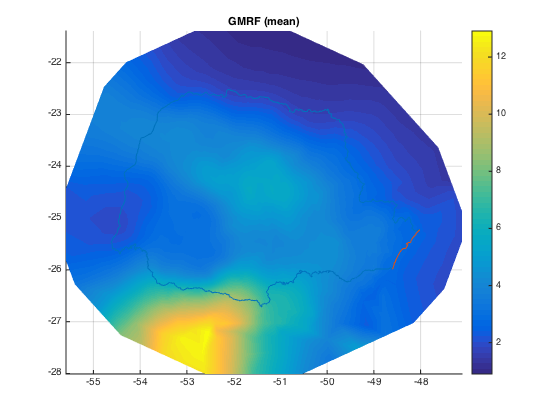
\includegraphics[width=5cm, height=4cm]{mesh_mean_obs.png} }}%
  \qquad
  \subfloat[]{{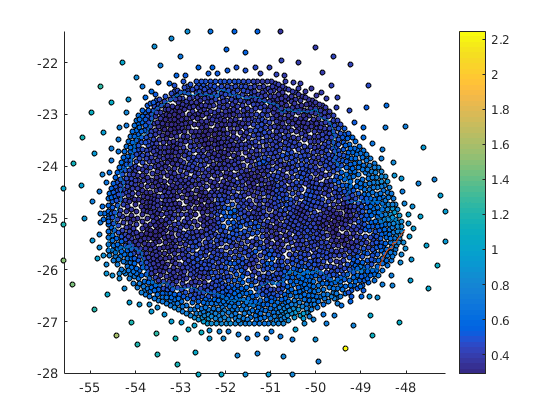
\includegraphics[width=5cm, height=4cm]{mesh_mean_obs_se.png} }}%
  \caption{(a): Mean precipitation for mesh locations. (b): SE of mean precipitation for mesh locations.}
\label{fig:mesh}
\end{figure}

To construct the uncertainty for the predictions however, we sample $\txsample$ from the Gaussian approximation of its posterior $p_G(\btx|\by, \btheta)$. The precipitation observations are sampled 100 times according to the data model as $\Gamma(b, b^{-1} \exp(\btA \txsample))$. The median precipitation and the standard error are plotted in figure \ref{fig:meshpred}.
\begin{figure}[ht]
\centering
  \subfloat[]{{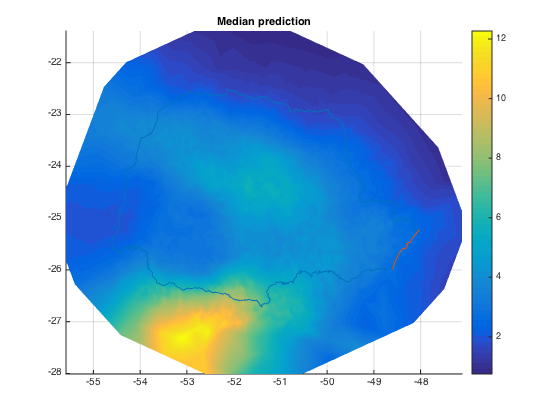
\includegraphics[width=5cm, height=4cm]{median_sim_y.png} }}%
  \qquad
  \subfloat[]{{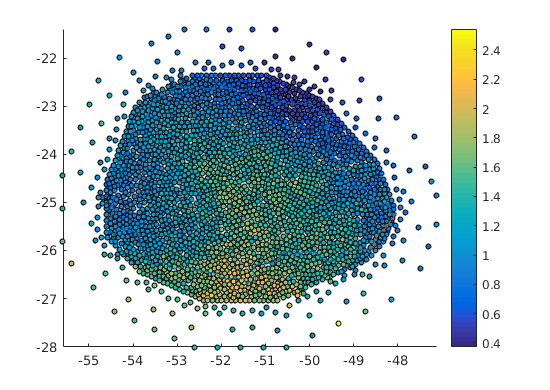
\includegraphics[width=5cm, height=4cm]{se_sim_y.png} }}%
  \caption{(a): Median precipitation (prediction). (b): SE of the predictions.}
\label{fig:meshpred}
\end{figure}
\section{Conclusions}

\end{document}
